% *** TODO:  Remove xii from bottom of last page of TOC

%%% Call as normal for book
%%% Call with kebonly=true (or set to anything) for ebook header stuff only.

%%% Define values we use throughout
\def\ktitle{$title$}
\def\ktitlelc{$title$}
\def\kisbnthirteenpb{999-8-7777777-66-1}
\def\kisbnthirteenkindle{999-8-7777777-66-2}
\def\klccn{2030101999}
\def\kpress{My Press}
\def\kauthor{Steinbeck Hemingway Faulkner III}
\def\kartist{Rembrandt Picasso Dali}

%%% Define the document class
\ifx \kebonly \undefined
\documentclass[10pt,twoside,openright]{memoir}
\else
\documentclass[10pt,oneside,openany]{memoir}	% If for ebook, onesided.  
\fi
\usepackage{mathpazo}
\usepackage[T1]{fontenc}
\usepackage{textcomp}
\usepackage{amssymb}
\usepackage[artemisia]{textgreek}
\usepackage{url}
\usepackage{hyperref}
\usepackage{graphicx}
\usepackage{array}
\usepackage{wrapfig}
\usepackage[object=vectorian]{pgfornament}
\usepackage[pass]{geometry}

% Set Stock size
\setstocksize{8in}{5in}

% Set \paperheight and \paperwidth.  Since trimsize=stocksize, no \settrims command is necessary to center the trimblock in the stockblock
\settrimmedsize{\stockheight}{\stockwidth}{*}

% Set \textwidth and \textheight
\settypeblocksize{6.2in}{3.2in}{*}

% Set the spine margin (\spinemargin)  The edge margin is then computed automatically
% Set the upper margin (\uppermargin).  The lower margin is then computed automatically
\ifx \kebonly \undefined
\setlrmargins{*}{0.8in}{*}
\setulmargins{*}{1in}{*}
\else		% If for ebook, use identical margins.
\setlrmargins{*}{0.9in}{*}
\setulmargins{*}{0.9in}{*}
\fi

% Set the footer (page number) positioning.  Footskip is distance from bottom of textblock to the top of the footer
\setlength\footskip{30pt}

% Flush bottom is unnecessary for poetry and we could use raggedbottom instead, but keep it safe just in case
\flushbottom

% Verify and accept layout.  
\checkandfixthelayout[fixed]

%%% Define macros used in poems
\def\kskip{\vskip 12pt}
\def\knewpage{\newpage}		% pagebreak causes previous page to spread.  newpage leaves blank at bottom
\newcommand{\kenmulticol}[1]{#1}
\newcommand{\kchapname}{}
\newcommand{\kfootarrow}{}
\def\klinebreak{\linebreak}
\def\kblankpage{ % Useful macro to insert a blank page (no page number), for front or rear matter
\newpage
\thispagestyle{empty}
\mbox{}
}

%%% We want a small arrow on odd continuation pages (except the first) of a piece, so the reader
%%% knows it doesn't end there.  \pbarrow is the arrow, and we use the footer style to put it only on 
%%% odd non-chapter pages.  We don't use \chapter, but we do still end up with chapter as the relevant pagestyle
%%% somehow.  If this ever stops working we can explicitly set the pagestyle to that in \kunit
\def\pbarrow{\renewcommand{\kfootarrow}{$\triangleright$}}	

%%% Default spec, but this gets overridden almost everywhere (the true defaults appear in GenInputs.py and the kenflash and kenpoem macros below)
\parindent 0pt
\parskip 0pt
\linespread{1.35}	% Big, but the right choice for poetry/flash-fiction with Palladio/Palatino

%%% Chapter/section defs.  We don't use chapters, so skip that one. The rest are used for my own formatting purposes (via markdown).
\renewcommand{\chapter}[1]{}	% Disable
\renewcommand{\section}[1]{\knewpage}	% ## is a forced newpage
\renewcommand{\subsection}[1]{\kskip}	% ### is a stanza break
\renewcommand{\subsubsection}[1]{	% #### is a bold/centered flourish/etc
\kskip
\begin{center}\textbf{#1}\end{center}
\kskip
}

%%% For the actual pieces, we use kenflash and kenpoem, both of which wrap kenunit with the appropriate parms.
% kenunit takes args:  title, linespread, parskip, parindent, vskip
% Do NOT remove the blank lines from this script!!!  The formatting gets screwed up if you do that!
\newcommand{\kenunit}[6]{ %
{{\LARGE\textbf{#1}}
\vskip 0.25 in
\pbarrow
\addcontentsline{toc}{chapter}{#1}
\renewcommand{\kchapname}{#1}
\addtocounter{kchapcnt}{1}
\parskip #3
\parindent #4
\vskip #6
\fontsize{10pt}{10pt}\selectfont
\linespread{#2}\selectfont

\input #5

}}

% kenpoem takes args:  title, file, linespread, vskip
\newcommand{\kenpoem}[4] { \renewcommand{\subsection}[1]{\vskip 12pt} \kenunit{#1}{#3}{0pt}{0pt}{#2}{#4} }

% kenflash takes args:  title, file, linespread, vskip
\newcommand{\kenflash}[4] { \renewcommand{\subsection}[1]{} \kenunit{#1}{#3}{12pt}{0pt}{#2}{#4} }

% kenflash takes args:  title, file, linespread, vskip
\newcommand{\kenstory}[4] { \renewcommand{\subsection}[1]{} \kenunit{#1}{#3}{0pt}{12pt}{#2}{#4} }

%%% Set header/footer styles.  We use a slightly-ornamented, centered page number in the footer
%%% and no header at all.  We also use this to implement the continuation arrows where needed.
\copypagestyle{chapter}{plain}
\makeevenfoot{chapter}{}{$\cdot$\hskip3pt{\fontfamily{ppl}\footnotesize\selectfont\thepage}\hskip3pt $\cdot$}{}
\makeoddfoot{chapter}{}{$\cdot$\hskip3pt{\fontfamily{ppl}\footnotesize\selectfont\thepage}\hskip3pt $\cdot$}{}
\makeevenfoot{plain}{}{$\cdot$\hskip3pt{\fontfamily{ppl}\footnotesize\selectfont\thepage}\hskip3pt $\cdot$}{}
\makeoddfoot{plain}{}{$\cdot$\hskip3pt{\fontfamily{ppl}\footnotesize\selectfont\thepage}\hskip3pt $\cdot$}{\kfootarrow{}}

%%% Chapter counter for TOC
\newcounter{kchapcnt}
\setcounter{kchapcnt}{1}

%%% Don't allow hyphenation if just 2 chars
\emergencystretch=15pt
\hyphenpenalty=500
\righthyphenmin=4
\lefthyphenmin=4

%%% TOC should only contain top level entries
\settocdepth{chapter}

%%% Macros for adverts.  Each advert page has a top and bottom (or just top) advert.  
%%% The line between them and vertical spacing is external to these and we must tweak the vertical spacing as needed.
%%% Used in the end-matter
\newcolumntype{C}[1]{>{\centering\let\newline\\\arraybackslash\hspace{0pt}}m{#1}}
\newcolumntype{L}[1]{>{\let\newline\\\arraybackslash\hspace{0pt}}m{#1}}

\newcommand{\kadverttop}[3]{%
\begin{minipage}[c][][t]{\textwidth}
\renewcommand{\subsection}[1]{\vskip 12pt} 
\parskip 12pt
\parindent 0pt
\begin{center}
\pagestyle{empty}
\fontsize{8pt}{8pt}\selectfont
\begin{center}\textbf{\textsc{#1}}\end{center}
\vskip 12pt
\begin{tabular}{C{1.5in} L{1.6in}}
\includegraphics[width=\linewidth]{#2} & 
\input #3
\end{tabular}
\end{center}
\end{minipage}
}

\newcommand{\kadvertbot}[4]{%
\begin{minipage}[c][][b]{\textwidth}
\renewcommand{\subsection}[1]{\vskip 12pt} 
\parskip 12pt
\parindent 0pt
\begin{center}
\fontsize{8pt}{8pt}\selectfont
\begin{center}\textbf{\textsc{#1}}\end{center}
\vskip 12pt
\begin{tabular}{C{1.5in} L{1.6in}}
\includegraphics[width=\linewidth]{#2} &  
\input #3
\end{tabular}
\vglue #4
\noindent\textbf{Available through Amazon, B\&N, and bookstores everywhere.}
\end{center}
\end{minipage}
}

%%% Begin the actual book
\begin{document}
\pagestyle{empty}	% No header/footer for frontmatter

%%% Front-matter:  Title, halftitle, copyright, toc, etc.
\frontmatter

%%% Half-title page (recto)
\newpage
\begin{center}
\begin{vplace}[0.5]
\fontsize{14pt}{14pt}\selectfont
\textsc{\ktitlelc}
\end{vplace}
\end{center}

%%% Blank page (verso)
\kblankpage

%%% Title Page (recto)
\newpage
\vskip 2in
\begin{center}
\fontsize{12pt}{12pt}\selectfont
\begin{tabular}[c]{c}
\\
\\
\\
\\
\\
\\
\\
\LARGE\textsc{\ktitlelc}\\
\\
\\
\\
\\
\\
\\
\large A collection
\\
\large of Mixed Works\\
\\
\large by\\
\\
\large \kauthor\\
\\
\\
\\
\\
\\
\\
{\large \kpress}
\end{tabular}
\end{center}

%%% Copyright Page (verso)
\newpage
\begin{center}
\fontsize{8pt}{8pt}\selectfont
\begin{tabular}[c]{l}
\\
\\
\\
\\
\\
\\
\\
\\
\\
\\
\\
Copyright \copyright\, 2021 by \kauthor\\
\\
All rights reserved.\\
\\
ISBN-13 (paperback): \kisbnthirteenpb\\
\\
ISBN-13 (ebook): \kisbnthirteenkindle\\
\\
Library of Congress Control Number: \klccn\\
\\
Published by \kpress\\
\\
Printed in the United States of America\\
\\
Cover Art by \kartist\\
\\
First Edition\\
\\
\\
\end{tabular}
\end{center}

%%% TOC (starts recto, but multipage)
\renewcommand{\contentsname}{}
\pagestyle{empty}
\newpage
\begin{center}
\LARGE\textsc{contents}
\end{center}
\vskip -28pt
\thispagestyle{empty}
\renewcommand*{\cftchapterfont}{\normalfont}
\renewcommand*{\cftchapterpagefont}{\fontfamily{ppl}\selectfont}
\setlength{\beforechapskip}{-12pt}
\addtocontents{toc}{\protect\thispagestyle{empty}}
\tableofcontents*
%\clearpage

%%% The poems
\openany
%\kblankpage
\pagestyle{plain}
\mainmatter
\input inputlist.tex

%%% Deactivate the footer turn-arrow for back-matter (but probably unnecessary since empty pagestyle)
\renewcommand{\kfootarrow}{}

%%% Begin the backmatter
\backmatter

%%% Call to action page (recto)
\newpage
\pagestyle{empty}
\begin{center}
\fontsize{12pt}{12pt}\selectfont
\begin{tabular}[c]{c}
\\
\\
\\
Thank you for reading \\
\textit{\ktitle}\\
\\
If you liked it,\\
please consider \\
writing a review on \\
\textbf{Amazon} or \textbf{Goodreads}\\
\\
{\resizebox{0.6\linewidth}{1.2ex}
    {{%
    {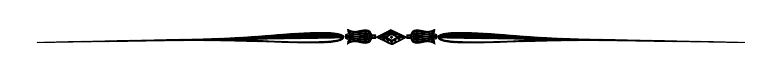
\begin{tikzpicture}
    \node  (C) at (0,0) {};
    \node (D) at (9,0) {};
    \path (C) to [ornament=89] (D);
    \end{tikzpicture}}}}}%
\\
\\
Sign up for my newsletter\\
at \textbf{www.mywebsite.com}\\
for information about\\
upcoming books and projects!\\
You will get exclusive\\
access to goodies such as\\
free chapters, stories,\\
and entry into a raffle to win\\
a set of books! \\
\\
{\fontsize{16pt}{16pt}\selectfont\textbf{www.mywebsite.com}}\\
\end{tabular}
\end{center}

%%% Blank page (verso)
\kblankpage

%%% Start Advert pages
\newpage
\savegeometry{Mem}
\newgeometry{top=28pt,bottom=0pt}
\pagestyle{empty}
\begin{Spacing}{1.1}

%%% Advert page 1 (recto)
\kadverttop{My First Book}{book1.bw.jpg}{book1_blurb.tex}
\vskip 20pt
\begin{center}\rule[0.5ex]{0.8\textwidth}{1pt}\end{center}
\vskip 12pt
\kadvertbot{My Second Book}{book2.bw.jpg}{book2_blurb.tex}{8pt}

%%% Blank page (verso)
\kblankpage

%%% End advertising pages
\end{Spacing}
\loadgeometry{Mem}

%%% Acknowledgments (recto)
\newpage
\input{ack.tex}

%%% Blank page (verso)
\kblankpage

%%% About the author page (recto)
\newpage
\input{about.tex}

%%% Blank page (verso)
\kblankpage

%%% Extra blank pages to get to x4 or x6 page count
\kblankpage
\kblankpage
\kblankpage

\end{document}


